\chapter{Анализ проблематики задачи геолокации по изображениям}
\label{chapter1}
\begin{comment}
Это обзорно-аналитическая глава, в которой требуется отразить:

\begin{itemize}
	\item результат изучения различных существующих методов решения задач в рамках проблематики УИРа/диплома (иногда даже в смежных областях), это обзорный аспект, который пишется, в основном, на основе имеющейся литературы или/и программного обеспечения;
	\item сравнение (с какой-либо определенной целью) этих методов и средств.
\end{itemize}
\end{comment}

%Большие отсупы --- это хорошо. Облегчает чтение длинных <<простыней>> текста
\section{Обзор методов геолокации по изображениям}

Задача определения места съемки фотографии довольно непроста из-за неоднозначности и недостаточности информации, содержащейся в одном изображении. Например, типичная пляжная сцена (море, солнце, песок, небо...) может быть заснята почти в любой точке земли. Даже достопремечательности не всегда могут служить абсолютными ориентирами: Эйфелева башня может указывать на Париж с Елисейскими полями, а может на Лас-Вегас или на село Париж в Челябинской области. В отсутствие подобных ориентиров люди полагаются на такие признаки как язык дорожных знаков, разметку, окружающую флору; опираясь на знания о внешнем мире для уточнения оценки местоположения. Традиционные системы компьютерного зрения часто не обладают подобными сведениями, полагаясь лишь на то что можно почерпнуть из тестовой выборки.

Для решения задачи геолокации применялись:
\begin{itemize}
	\item расстояния между изображениями вычисляемые при помощи глобальных дескрипторов изображений. Рассматривалось в 2008 году  в работе \texttt{IM2GPS} Хейса и Эфроса из Карнеги Меллон \cite{im2gps}.
	Рассматривается далее более подробно.
	\item Дополнение данными спутниковой съемки \cite{lin2013cross}. 
	\item Распознавание ориентиров \cite{avrithis2010retrieving}.
	\item Распознавание формы городского горизонта Skyline2GPS \cite{ramalingam2010skyline2gps}
\end{itemize}

\section{Изучение и сравнительный анализ алгоритмов глубокого обучения с целью выбора подхода к задаче}

Для задач обработки изображений используется множество различных методов. Перечислим некоторые из них.

\subsection{Глобальные дескрипторы}

Глобальные дескрипторы описывают изображение в целом и представляют его в виде векторов признаков. Обычно каждая точка вносит вклад в значение дескриптора.
При поиске по коллекции цветных изображений для человека одной из наиболее значимых характеристик является цвет. К тому же он инвариантен относительно расположения объектов и размера изображения, что упрощает его анализ. Самое распространенное представление цвета - это цветовая гистограмма \cite{colorhist_2018} (гистограмма
распределения цветов). Подход заключается в том, что цветовое пространство разбивается
на промежутки и для каждого промежутка вычисляется доля пикселей из данного
промежутка. Процесс разбиения цветового пространства на ограниченное количество
цветовых диапазонов называется квантованием. Сложность данного подхода заключается
в построении такого разбиения, чтобы цвета из одного диапазона были плохо различимы
человеком, а цвета из разных диапазонов, наоборот, различались. Пример гистограммы с
квантованием в цветовом пространстве RGB изображен на Рисунке \ref{pic:exchist}.


\begin{figure}%
	\begin{center}
		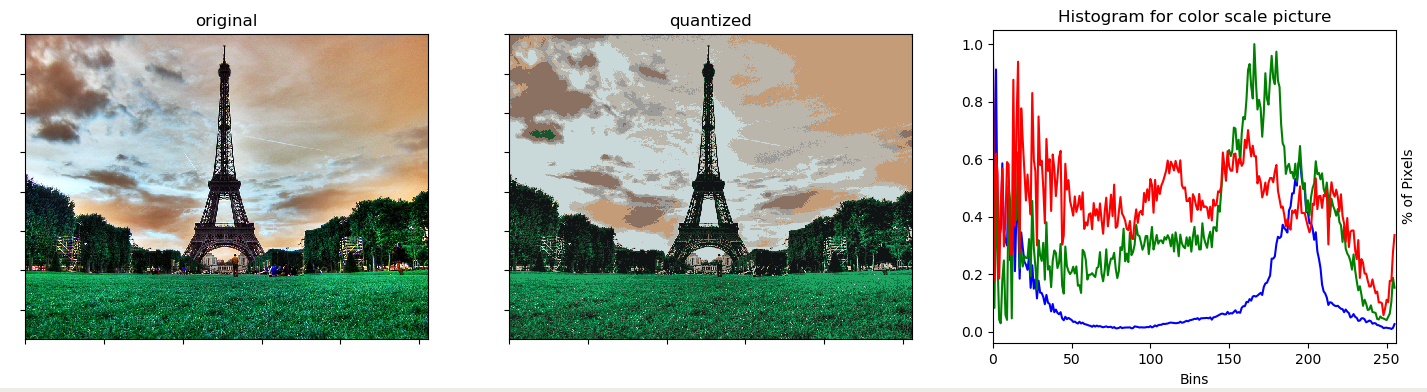
\includegraphics[width=.9\columnwidth]{./img/hist_0}%
	\end{center}
	\caption{Гистограмма цветов и квантованная картинка.\\ Квантование проведено с помощью 10-NN кластеризации}%
	\label{pic:exchist}%
\end{figure}


В простейшем случае, и в частности в данном примере, не учитывается
пространственное расположение цветов на изображении. Решением является разбиение
изображения на фиксированные блоки и вычисление цветовой гистограммы отдельно для
каждого блока. Однако в данном решении возникает проблема в подборе размеров блоков.
Еще одним решением проблемы учета пространственного расположения цветов является
модификация классической цветовой гистограммы HistSP [4]. Главная идея данного
метода заключается в том, что для каждого ненулевого элемента гистограммы 
вычисляется центр масс пикселей соответствующего цвета, его координаты сохраняются в
числе элементов вектора признаков.
Альтернативная модель представления цвета изображения – это цветовые
моменты, предложенные Stricker M., Orengo M. в [5,6]. Авторы рассматривают
распределения отдельных цветовых каналов как части трехмерного распределения.
Вводится пять фиксированных областей: центральная область в виде эллипса и четыре
боковые области (Рисунок 2). Для каждой области вычисляется математическое ожидание
по каждому из цветовых каналов и попарные ковариации распределений каналов. Для
каждого из пикселей вычисляется его степень принадлежности к области: чем ближе к
границе области, тем меньше степень принадлежности к ней. Это значение регулирует
вклад цвета соответствующего пикселя в общую оценку распределения цвета области.
Еще одной значимой характеристикой изображения является текстура. Она
описывает структуру объектов на изображении, и определяется по распределению уровня
яркости изображения.
Одним из наиболее известных представлений текстурных характеристик
изображения являются матрицы смежности (матрицы совместного распределения яркости
на изображении - Grey Level Co-occurrence Matrices, GLCM) [7]. Матрица смежности
зависит от разницы яркостей в соседних пикселях. По ней можно вычислить значения 
различных статистических показателей, например, таких как энтропия (степень
неоднородности), контраст, показатель однородности, показатель гладкости и др.
Еще одними из известных текстурных признаков являются признаки Тамуры [8],
которые были выделены с учетом особенностей зрительного восприятия человека. Они
включают в себя зернистость, контрастность, направленность, линейность, регулярность и
грубость. Из них были определены три наиболее подходящих при решении задачи поиска
изображений – это зернистость, контрастность и направленность. Если собрать эти
значения в одно изображение, в котором red, green, blue каналы будут заменены на
зернистость, контрастность и направленность соответственно, то из полученного
изображения можно вычислить 3d текстурную гистограмму. Если будем разбивать на
промежутки зернистость, контрастность и направленность, то получим 3d гистограмму,
аналогичную цветовой 3d гистограмме на Рисунке 1, только с другими осями координат.
Для рассмотрения текстуры изображения в различных масштабах, можно
использовать вейвлет-анализ, который заключается в разложении сигнала по базисным
функциям. Базисные функции (вейвлеты) строятся на основе порождающего вейвлета с
помощью сдвига и масштабирования. Берется исходное изображение и строится первая
проекция сигнала (свертка с первой базисной функцией), потом вычисляется разность
исходного сигнала с полученным и строится вторая проекция этой разности (свертка со
второй базисной функцией), и т.д. Причем, каждая базисная функция является сдвигом
предыдущей, растянутой в 2n
раз (n характеризует масштаб). Таким образом, в итоге
получаем грубую версию изображения. Такие базисные функции обычно называют
фильтрами. Одними из эффективных и используемых фильтров являются фильтры Габора
[9], ICA-фильтры (Independent Component Analysis, ICA [10]). ICA-фильтры получены
путем анализа обучающего множества изображений. Данные фильтры являются
локальными и подобны фильтрам Габора, однако в отличие от них носят естественный
характер и отражают основные направления текстуры изображений, по которым они
строились. Также проводились исследования, показывающие, что способ построения ICA-
фильтров схож с процессом зрительного обучения человека.
Еще одним важным признаком для сравнения изображений является форма
объектов. Простейшими признаками являются центр тяжести фигур, площадь,
направление главной оси и т.д. Существуют и более сложные методы, представляющие
фигуры более детально, их можно разделить на два класса:
\begin{itemize}
\item  внешнее представление, основанное на информации о контуре фигуры –
дескрипторы границ, к ним относятся разные виды сигнатур, дескрипторы
Фурье, вейвлет-дескрипторы, цепные коды и т.д.;
\item  внутреннее представление, основанное на информации о фигуре в целом –
дескрипторы областей, к ним относятся, например, инварианты моментов и т.д.
\end{itemize}
Более подробно цветовые признаки, текстурные признаки и признаки формы описаны в
\subsection{Локальные дескрипторы}

Локальные дескрипторы представляют собой вектора признаков, построенные по
отдельным фрагментам изображения. То есть они не описывают все изображение, а
содержат информацию только о выбранных некоторым способом фрагментах. Самыми
известными локальными дескрипторами являются SIFT \cite{lowe1999sift} (Scale Invariant Feature
Transform), SURF \cite{bay2006surf} (Speeded Up Robust Features), PCA-SIFT \cite{ke2004pcasift} (PCA – Principal
Component Analysis) и т.д.
Метод SIFT (Scale Invariant Feature Transform) обнаруживает и описывает
локальные особенности изображения. Получаемые с помощью него признаки
инвариантны относительно масштаба и поворота, устойчивы к ряду аффинных
преобразований, шуму, изменению в освещении. Данный алгоритм можно разделить на
две части: определение «точек интереса» (key points, points of interest, salient points) и построение дескрипторов окрестностей данных точек. Существует несколько способов
определения точек интереса. Алгоритм, предложенный в рамках SIFT, один из самых
известных. Он заключается в использования пирамиды Гаусса [14], которая строится для
изображения. Далее изображения приводятся к одному размеру, и вычисляется их
разность (DoG, difference-of-Gaussian images). Причем в
качестве кандидатов точек интереса выбираются только те пиксели, которые сильно
отличаются от остальных, это делается, например, путем сравнения каждого пикселя
изображения с несколькими соседними данного масштаба, с несколькими
соответствующими соседями в большем и меньшем масштабе. 
Далее для каждой такой точки интереса вычисляется локальный дескриптор,
характеризующий направление градиентов в пикселях некоторой окрестности. Главным
минусом SIFT дескрипторов является их высокая размерность и большое количество на
изображении. PCA-SIFT \cite{ke2004pcasift} (PCA, Principal Component Analysis – анализ главных
компонент) дескриптор – одна из вариаций SIFT, в которой уменьшается размерность
дескриптора с помощью анализа главных компонент. Это достигается с помощью
нахождения пространства собственных векторов, на которое впоследствии проецируются
вектора признаков.
Альтернативным подходом является SURF [12] (Speeded Up Robust Features),
который в несколько раз быстрее SIFT. В данном подходе для ускорения поиска точек
интереса используются интегральные изображения [15]. Значение в каждой точке
интегрального изображения вычисляется как сумма значения в данной точке и значений
всех точек, которые находятся выше и левее данной. С помощью интегральных
изображений за константное время вычисляются так называемые прямоугольные фильтры
[16], которые состоят из нескольких прямоугольных областей. SURF в несколько раз
быстрее SIFT, менее чувствителен к шуму, к повороту, но чувствителен к изменению
освещения или угла, под которым был сделан снимок.
Глобальные и локальные дескрипторы обычно используются для решения разных
задач. Глобальные дескрипторы в основном применяются для решения задачи общего
поиска изображений по содержанию, то есть для поиска по запросу-образцу визуально и
семантически похожих изображений. В данном случае важно все изображение в целом, а
не отдельные его области, поэтому для решения данной задачи подходят глобальные
дескрипторы, характеризующие все изображение. Локальные дескрипторы обычно
применяются для решения задачи поиска нечетких дубликатов. Дубликатами считаются 
изображения одной и той же сцены или объекта, сделанные в разных условиях или
разного качества, в частности, изображения одной и той же сцены в разном масштабе или
снятые с разных точек, с различием в освещении или с незначительными изменениями
фона. При решении данной задачи важно обнаружить сходство отдельных частей
изображений, для данных целей обычно применяются локальные дескрипторы,
описывающие особенности областей изображений.
Все вышеописанные локальные дескрипторы используют общую парадигму,
заключающуюся в нахождении точек интереса и построении для каждой из них
дескриптора, описывающего ее окрестность. Принципиально другой подход описан в
работе \cite{localselfsim}. Он основан на свойстве повторяемости (самоподобии) фрагментов на
изображении, то есть на наблюдении, что небольшие фрагменты изображения имеют
свойство повторяться на нем в том же или другом масштабе. Информация о такой
повторяемости в пределах некоторой области изображения формирует так называемую
геометрическую разметку. С помощью данной геометрической разметки формируются
самоподобные локальные дескрипторы. Причем, даже если изображения имеют разную
текстуру, цвет и др., но их геометрические разметки похожи, то дескрипторы тоже будут
похожи. Эксперименты, проведенные авторами работы, показали применимость данных
дескрипторов для решения задач распознавания объектов и поиска фрагментов в
коллекциях изображений и видео без предварительного обучения. Также стоит заметить,
что большинство других локальных дескрипторов строятся только для точек интереса и,
следовательно, не описывают все изображение в целом. Самоподобные локальные
дескрипторы изначально строятся для каждой точки изображения, после чего
производится фильтрация, даже после которой самоподобные дескрипторы образуют
более плотное множество по сравнению с другими описанными локальными
дескрипторами.

\section{Анализ алгоритмов пространственного разбиения поверхности земли для решения задачи классификации }

Подразумевается что мы рассматриваем задачу геолокации как задачу классификации областей Земной поверхности, а не как задачу регрессии координат. Это позволяет работать с выходом модели как с гистограммой распределения вероятности нахождения фотографии в точках поверхности земли.
Достоинство такого подхода схоже с задачей классификации изображений, когда правильный класс может быть не первым, а например одним из 5 наиболее вероятных догадок, что может быть использовано.
Существует множество способов проекции $2$-сферы на плоскость, однако у каждого из них есть свои недостатки:
Проекция Меркатора, представитель класса равноугольных проекций, не сохраняет пропорций (Гренландия значительно меньше Африки), Равновеликие проекции не сохраняют форму объектов, что менее критично но также нежелательно.
Поэтому интересным представляется следующее решение проблемы --- использование не проекции  на плоскость, а разбиения поверхности на области при помощи проекции поверхности на грани куба, См рис \ref{pic:projection}.
\begin{figure}
	\centering
	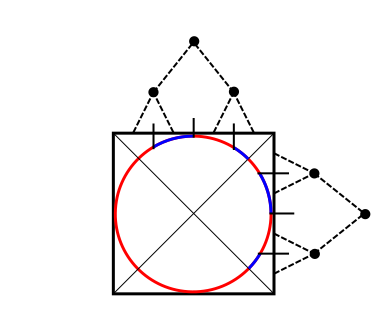
\includegraphics{img/projection}
	\caption{S-2 Проекция в двухмерном случае}
	\label{pic:projection}
\end{figure}

\section{Существующие решения задачи геолокации по изображениям}

Описанные выше в пункте по работы представляют собой state-of-the-art на текущий момент, однако автору не удалось обнаружить в свободном доступе ПО, демонстрирующее функциональность описанных методов.


\section{Анализ возможностей применения подхода transfer learning к проблеме геолокации с помощью глубокого обучения}


\section{Выводы}

Подразумевается что разрабатываемая система действует автономно и не обладает дополнительной информацией о мире кроме информации о пространственной плотности объектов тестовой выборки.

Тут пишем выводы по результатам анализа: что и с какой целью было проанализировано, какие выводы из этого сделаны, как они повлияли (должны повлиять) на дальнейший ход работы. Результаты анализа приводятся попунктно, основные вывода из проделанного анализа. Например:

\begin{enumerate}
	\item Выполнен сравнительный анализ таких-то формальных систем с точки зрения применимости к решению такой-то задачи. Ни одна из проанализированных напрямую не подходит, поэтому требуется разработать вариацию на основе системы такой-то.
	\item Были проанализированы варианты программных архитектур на основе систем. С учетом требований к поддержке больших объемов данных и высоких требований к потенциалу модернизируемости, была выбрана за основу такая-то архитектура.
	\item Сравнительный анализ таких-то библиотек показал, что библиотека X проще в использовании, но менее производительна, в то время как библиотека Y обеспечивает высокую производительность, но и требует значительных трудозатрат для использования. В связи с такими-то соображениями были принято решение использовать такую-то библиотеку.
\end{enumerate}



\section{Постановка задачи дипломной работы/курсового проекта}

Это всегда последний пункт. Далее пишется постановка задачи, на основе выданного задания. Это должен быть связный текст в объеме до 1-1,5 страниц. В этом разделе необходимо раскрыть цели и задачи УИРа/диплома. 

